\section{HARDWARE RESULTS}

\subsection{Induction Motor}

\begin{figure}[H]
	\centering
	
\includegraphics[width=4.0in]{sections/section4/images/inductionMotor/revo.png}
	\caption{Image of Induction Motor}
\end{figure}

We are using a revo 3 phase induction motor with the following specifications:

\begin{table}[H]
	\centering
	\begin{tabular}{|c|c|}
		\hline
		\textbf{Parameter} & \textbf{Value} \\ \hline
		Power & 0.25 Hp or  \\ \hline
		Voltage & 415 V (L-L) RMS \\ \hline
		Current & 6.5 A \\ \hline
		Frequency & 50 Hz \\ \hline
		Speed & 1440 rpm \\ \hline
		Phase & 3 \\ \hline
	\end{tabular}
	\caption{Induction Motor Nameplate Details}
\end{table}



\subsection{F23879d Launchpad}

\begin{figure}[H]
	\centering
	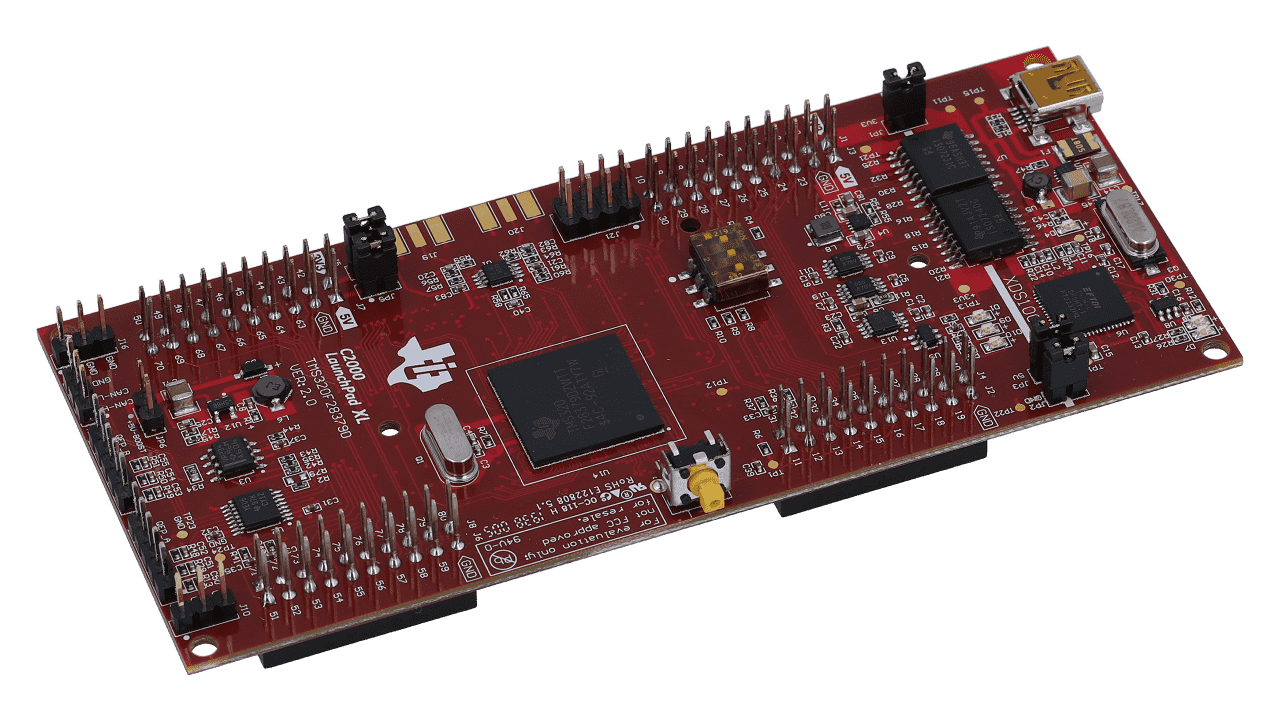
\includegraphics[width=4in]{sections/section4/images/f23879d/launchxl-f28379d-angled.png}
	\caption{Image of F28379D Launchpad}
\end{figure}


\subsection{Intelligent Power Module Fsam20sh60a}

\begin{figure}[H]
	\centering
	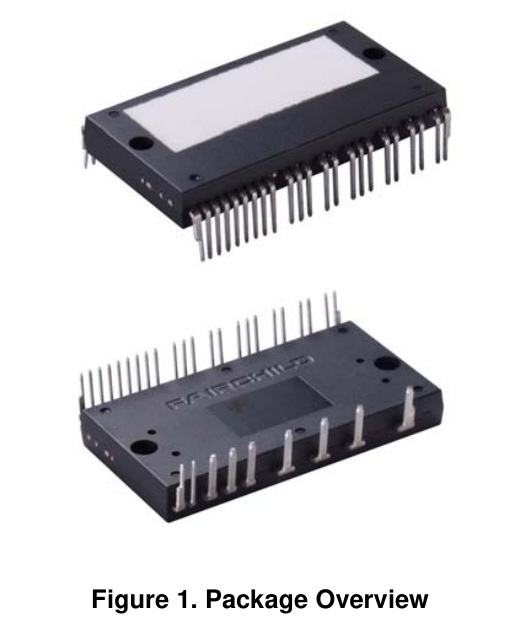
\includegraphics[width=3in]{sections/section4/images/IPM/ipm.png}
	\caption{Image of FSAM20SH60A module}
\end{figure}


We integrated the FSAM20SH60A, a Motion SPM® 2 module, as a fundamental component. This UL Certified (No. E209204 UL1557) device is a high-performance 3-phase IGBT inverter with integrated gate drivers and protection, proving to be an ideal solution for AC Induction, BLDC, and PMSM motors.

The FSAM20SH60A is designed with low-loss, short-circuit rated IGBTs, and an optimized gate drive to minimize EMI and losses. It also incorporates multiple on-module protection features such as under-voltage lockouts, over-current shutdown, thermal monitoring, and fault reporting, thus ensuring robust and reliable operation. 

One of the unique features of this module is its low thermal resistance achieved through the use of a ceramic substrate. It also includes separate open-emitter pins from low-side IGBTs for three-phase current sensing, supporting a wide variety of control algorithms. 

The FSAM20SH60A is tailored for a 15 kHz switching frequency and features a built-in NTC thermistor for accurate temperature monitoring. It operates on a single-grounded power supply and offers an inverter power rating of 1.5 kW at an input voltage range of 100~253 VAC. 

Moreover, the module provides an adjustable current protection level, allowing for customization via the selection of Sense-IGBT Emitter's external Rs. It also boasts an impressive isolation rating of 2500 Vrms per minute. 

The high-speed HVIC integrated into the FSAM20SH60A requires only a single supply voltage and effectively translates the incoming logic-level gate inputs to the high-voltage, high-current drive signals required to properly drive the module's internal IGBTs. 



\subsection{Pcb Design}

\begin{figure}[H]
	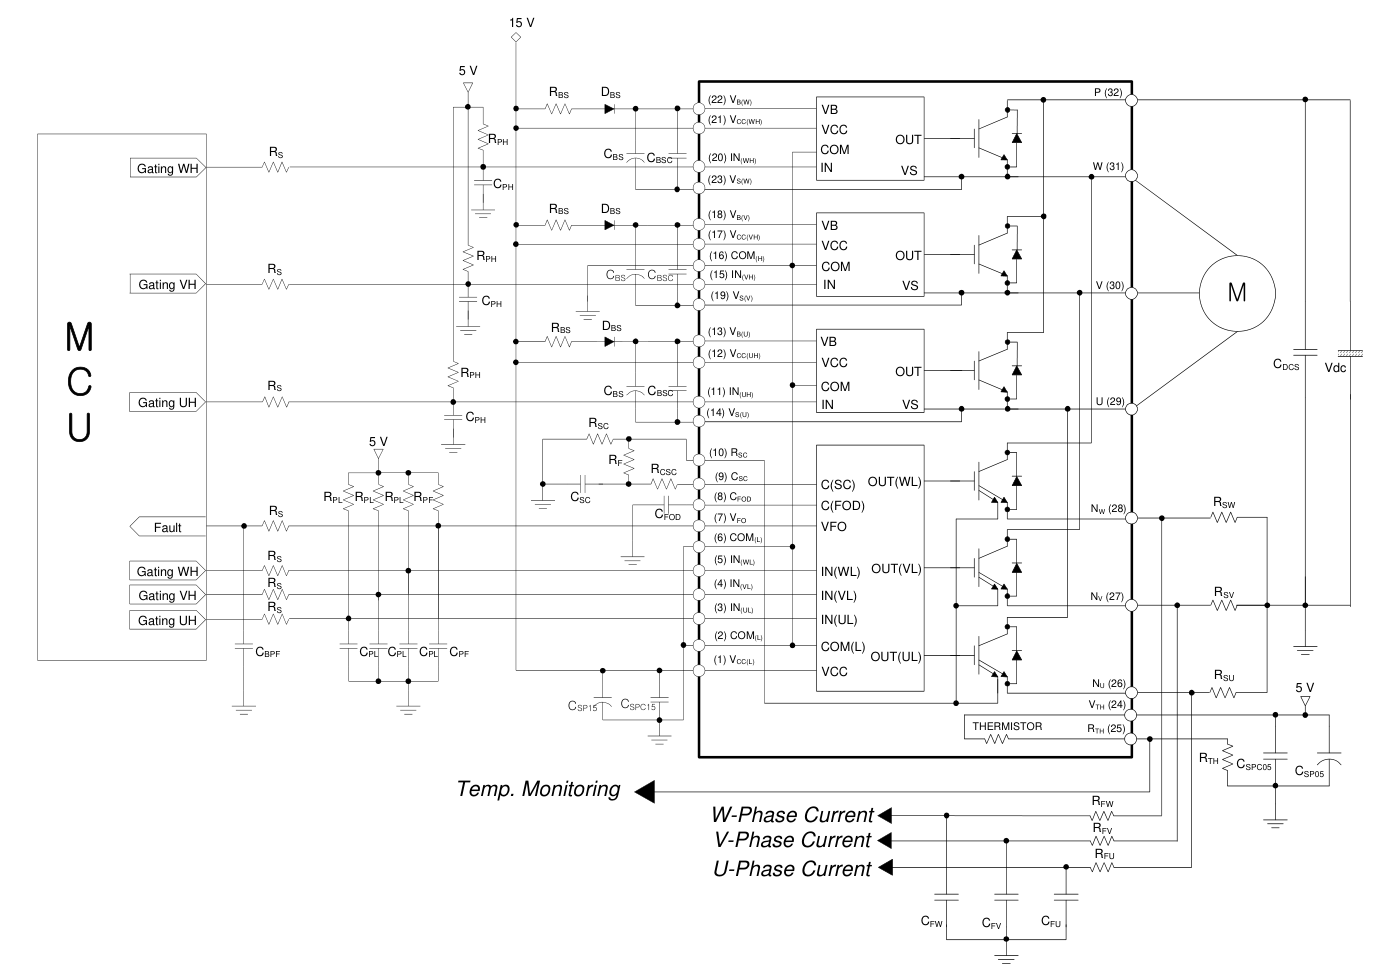
\includegraphics[width=6in]{sections/section4/images/PCBDesign/ApplicationCircuitfromDatasheet.png}
	\caption{Application Circuit from FSAM20SH60A Datasheet}
\end{figure}

In the PCB design section of our project, we developed a printed circuit board for the FSAM20SH60A, an intelligent power module. Our design strategy was primarily guided by the application circuit provided in the datasheet of the module. 

The application circuit served as a reference point for designing the PCB, ensuring that we adhered to the technical specifications and requirements of the module. In particular, we paid careful attention to the layout and routing of the circuit traces, the placement of components, and the thermal management considerations. 

The PCB design was optimized to facilitate the features and functions of the FSAM20SH60A. This included provisions for three-phase current sensing through separate open-emitter pins from low-side IGBTs, as well as accommodating the single-grounded power supply. 

Moreover, the design ensured the proper functioning of the built-in NTC thermistor for temperature monitoring, and the high-speed HVIC that requires only a single supply voltage. The layout also considered the adjustable current protection level, which can be customized via the selection of Sense-IGBT Emitter's external Rs. 

Software tools from National Instrument's circuit design suite were utilized to create the PCB layout. Multisim 14.3 was used for the schematic capture, while Ultiboard 14.3 was employed for the PCB layout design.

\begin{figure}[H]
	\centering
	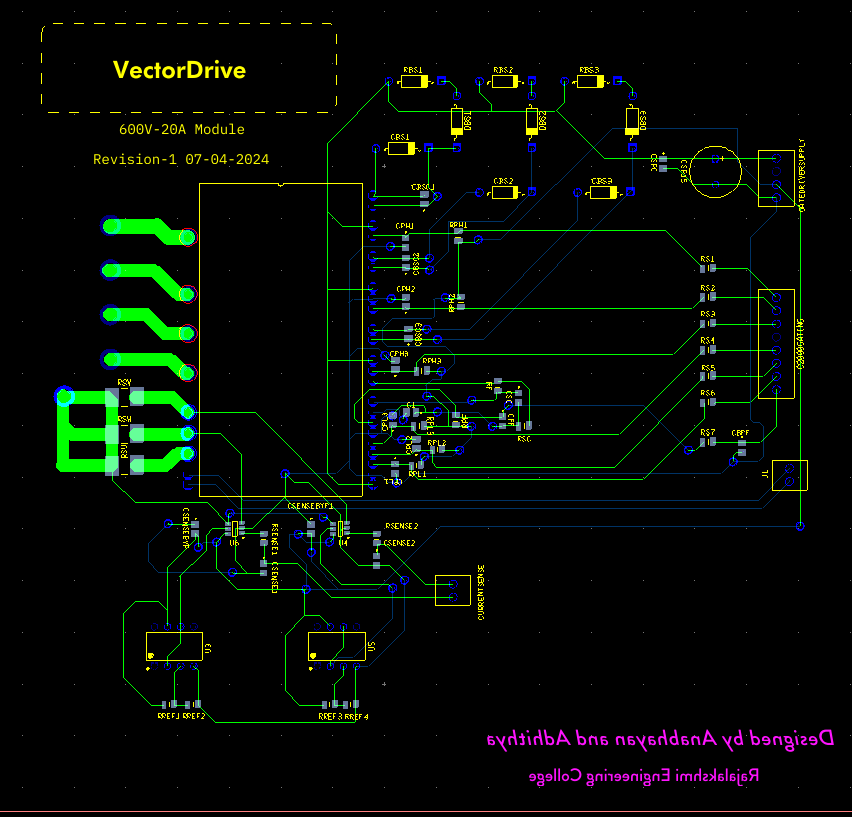
\includegraphics[width=4in]{sections/section4/images/PCBDesign/Ultiboard/Ultiboard.png}
	\caption{PCB Layout Design in Ultiboard}
\end{figure}


\begin{figure}[H]
	\centering
	
\includegraphics[width=3.5in]{sections/section4/images/PCBDesign/Ultiboard/3DTopView.png}
	\caption{3D View of PCB Layout Design in Ultiboard}
\end{figure}


\subsection{Current Measurement}

In our project, we implemented a strategy for current measurement using a shunt power resistor of 5 milli-ohms. This resistor was incorporated into two of the phase low pass filters, providing a reliable method for detecting and measuring the current flow.

Following the current detection, the signal was then directed to an IA182 operational amplifier. This component was crucial in amplifying the signal to a level suitable for further processing. The IA182 opamp was selected due to its high precision and stability, ensuring accurate amplification of the current signal.

Post amplification, the signal was fed into the Analog-to-Digital Converter (ADC) of the F28379D Launchpad. This conversion process transformed the analog current signal into a digital format, enabling the microcontroller to effectively interpret and utilize the data for further processing and control within the system. 


% Current sensing figure in multisim

\begin{figure}[H]
	\centering
	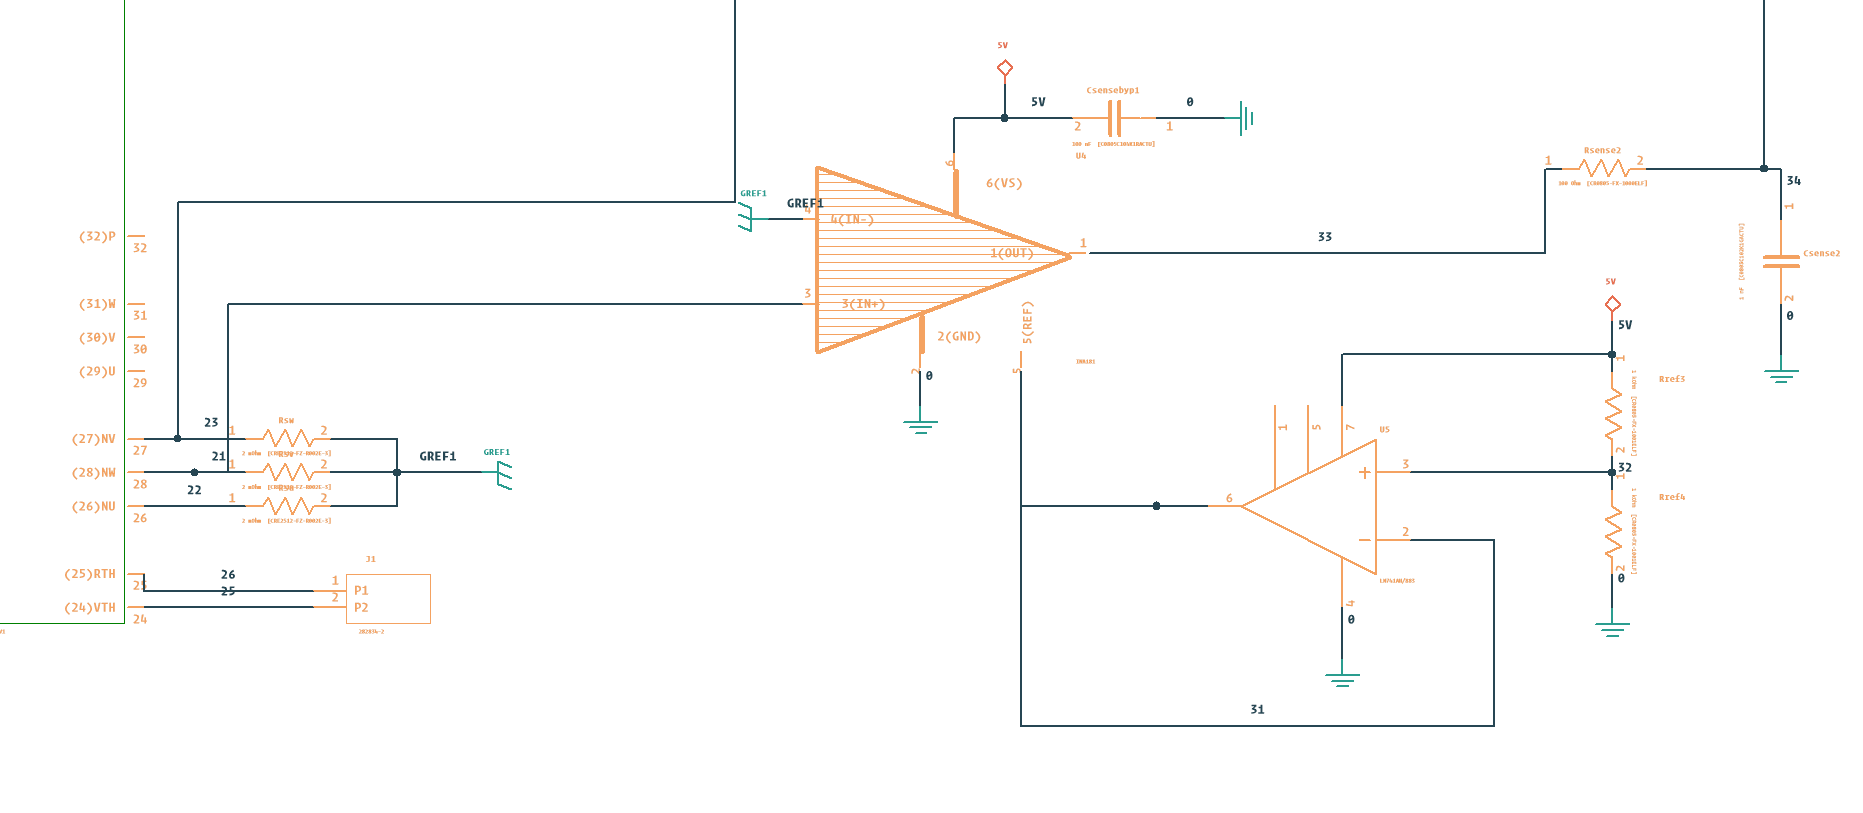
\includegraphics[width=6in]{sections/section4/images/PCBDesign/Multisim/MultisimCurrentSensing.png}
	\caption{Current Sensing Circuit in Multisim one of the phase is shown}
\end{figure}


\subsubsection{ADC CONFIG}


\newpage